\documentclass[a4paper, 12pt, oneside]{book}
\usepackage[italian]{babel} % Lingua italiana
\usepackage{authblk} % Per gli autori

\renewcommand\Authands{ e }

\title{Analisi empirica degli algoritmi di ordinamento}

\author[ ]{Graziano Francesco \thanks{Email: graziano.francesco@spes.uniud.it, Matricola: 166680}}
\author[ ]{Ongaro Michele \thanks{Email: ongaro.michele@spes.uniud.it, Matricola: 168049}}
\author[ ]{Petri Riccardo \thanks{Email: petri.riccardo@spes.uniud.it, Matricola: 167623}}
\author[ ]{Ungaro Marco \thanks{Email: ungaro.marco@spes.uniud.it, Matricola: 168934}}

\affil[ ]{Università degli Studi di Udine, Dipartimento di Matematica e Informatica}

\date{A.A. 2024-2025}
%\date{}

\usepackage{amsmath} % Per equazioni avanzate
\usepackage{amssymb} % Simboli matematici
\usepackage{graphicx} % Per immagini
\usepackage{lmodern} % Font simile a Computer Modern
\usepackage{geometry} % Per margini personalizzati
\usepackage{listings} % scrivere codice

\geometry{a4paper, margin=2.5cm}
\cleardoublepage
\pagestyle{plain}

\begin{document}

\maketitle % copertina del documento
\tableofcontents % sommario di tutti i titoli

\chapter*{Introduzione}
\addcontentsline{toc}{chapter}{Introduzione}


Il progetto richiede l'implementazione di quattro algoritmi di ordinamento per array interi di dimensioni variabili.
Gli algoritmi che andremo ad analizzare sono il Counting Sort, il Quick Sort, il Quick Sort 3 way e il Radix Sort (algoritmo a scelta).
Oltre alla corretta implementazione viene richiesto di effettuare un analisi empirica dei tempi medi di esecuzione degli algorimti al variare della dimensione dell'array e del range dei valori interi.
Per stimare i tempi di esecuzione di questi algoritmi garanantendo un errore relativo massimo pari a 0.001 adotteremo le seguenti metodologie:
\begin{itemize}
    \item Utilizzeremo un clock di sistema monotono per garantire precisione nelle misurazioni (ad esempio, \texttt{perf\_counter()} del modulo \(time\) in Python);
    \item Andremo a generare almeno 100 campioni per ciascun grafico, con i valori dei parametri (dimensione dell’array \(n\) e intervallo dei valori \(m\)) distribuiti secondo una progressione geometrica;
    \item Effettueremo più esecuzioni per ogni campione, per stimare in modo affidabile il tempo medio di esecuzione e, eventualmente, il relativo errore.
\end{itemize}
Dopo aver stimato i tempi di esecuzione per ciascun algoritmo, risulterà interessante confrontare i grafici ottenuti per analizzare il comportamento degli algoritmi in diverse situazioni, come il caso peggiore, quello migliore o in quello medio.

Da tutto questo potremmo ottenere una verifica empirica dell'andamento asintotico dei tempi di esecuzione di ogni algoritmo.


\chapter*{Counting Sort}
\addcontentsline{toc}{chapter}{Counting Sort}

Counting Sort è un algoritmo di ordinamento non comparativo, cioè che non ordina gli elementi confrontandoli tra loro come fanno invece altri algoritmi classici come QuickSort, Merge Sort o Bubble Sort.
Invece, conta quante occorrenze di ciascun valore sono presenti nell'array da ordinare e utilizza queste informazioni per posizionare gli elementi nell'array ordinato. Passaggi principali che effettua l'algoritmo:

\begin{enumerate}
    \item Determinazione del range: Identifica il valore massimo nell'array in input per determinare la dimensione necessaria dell'array di conteggio.
    \item Conteggio delle occorrenze: Crea un array ausiliario (\texttt{count}) in cui ciascun indice rappresenta un valore possibile dell'array originale, e si conta quante volte ciascun valore appare.
    \item Costruzione dell'array cumulativo: Trasforma l'array di conteggio in un array cumulativo, dove ogni elemento indica la posizione finale di un dato valore nell'array ordinato.
    \item Costruzione dell'array ordinato: Itera sull'array originale (in genere in ordine inverso per mantenere la stabilità), e si posiziona ogni elemento nella posizione corretta dell'array di output, decrementando il valore corrispondente nell'array di conteggio.
\end{enumerate}

\noindent L'algoritmo Counting Sort è particolarmente efficiente quando il range dei valori da ordinare è limitato rispetto alla dimensione dell'array.

\subsection*{Analisi della complessità}

La complessità temporale di Counting Sort è \(O(n + k)\), dove:

\begin{itemize}
    \item \(n\) è il numero di elementi nell'array da ordinare;
    \item \(k\) è il valore massimo presente nell'array.
\end{itemize}

\noindent Nel caso in cui si ha \(k=O(n)\) allora la complessità diventa \(O(n)\)

\subsection*{Grafico dei tempi di esecuzione}

Come prima cosa abbiamo generato il grafico in cui varia la lunghezza dell'array \textbf{n} mentre il range di valori che possono esserci nell'array rimane bloccato a 100000 (\(m=100000\)). Nel grafico qui sotto abbiamo come ascissa la variazione di \textbf{n} da 100 a 1000000 in scala scentifica dove ogni valore va moltiplicato per \(10^6\), come ordinata abbiamo il tempo in secondi di riordinamento dell'array.

\begin{center}
    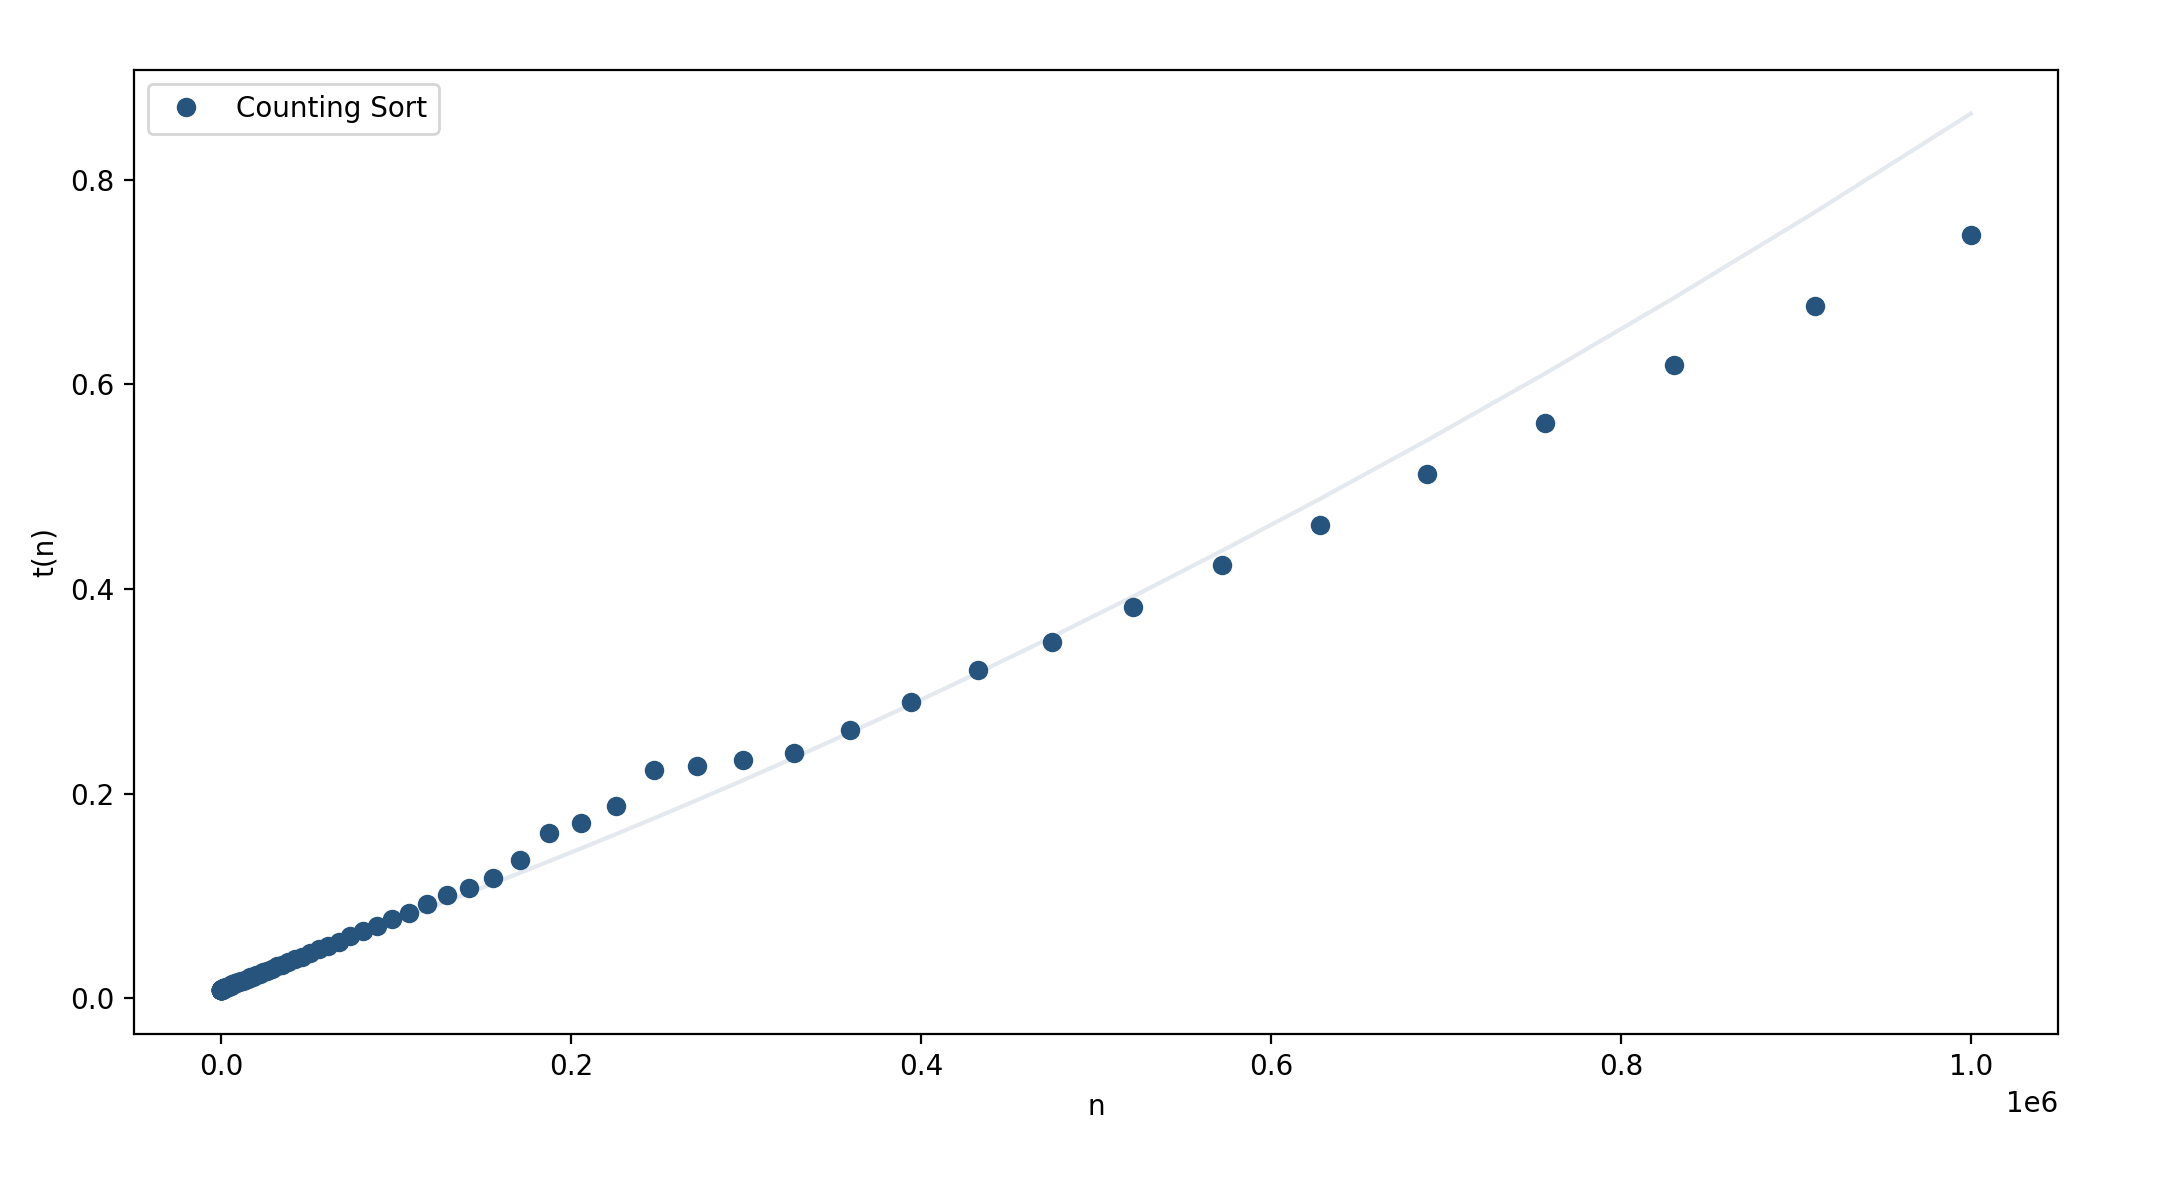
\includegraphics[width=0.9\textwidth]{images/grafico_counting_sort_n.png}
\end{center}    

\noindent Poi abbiamo generato il grafico in cui varia il range di valori che possono esserci nell'array \textbf{m} mentre la lunghezza dell'array rimane bloccata a 10000 (\(n=10000\)). Nel grafico qui sotto abbiamo come ascissa la variazione di \textbf{m} da 10 a 1000000 in scala scientifica, dove ogni valore va moltiplicato per \(10^6\), e come ordinata abbiamo il tempo in secondi di riordinamento dell'array.

\begin{center}
    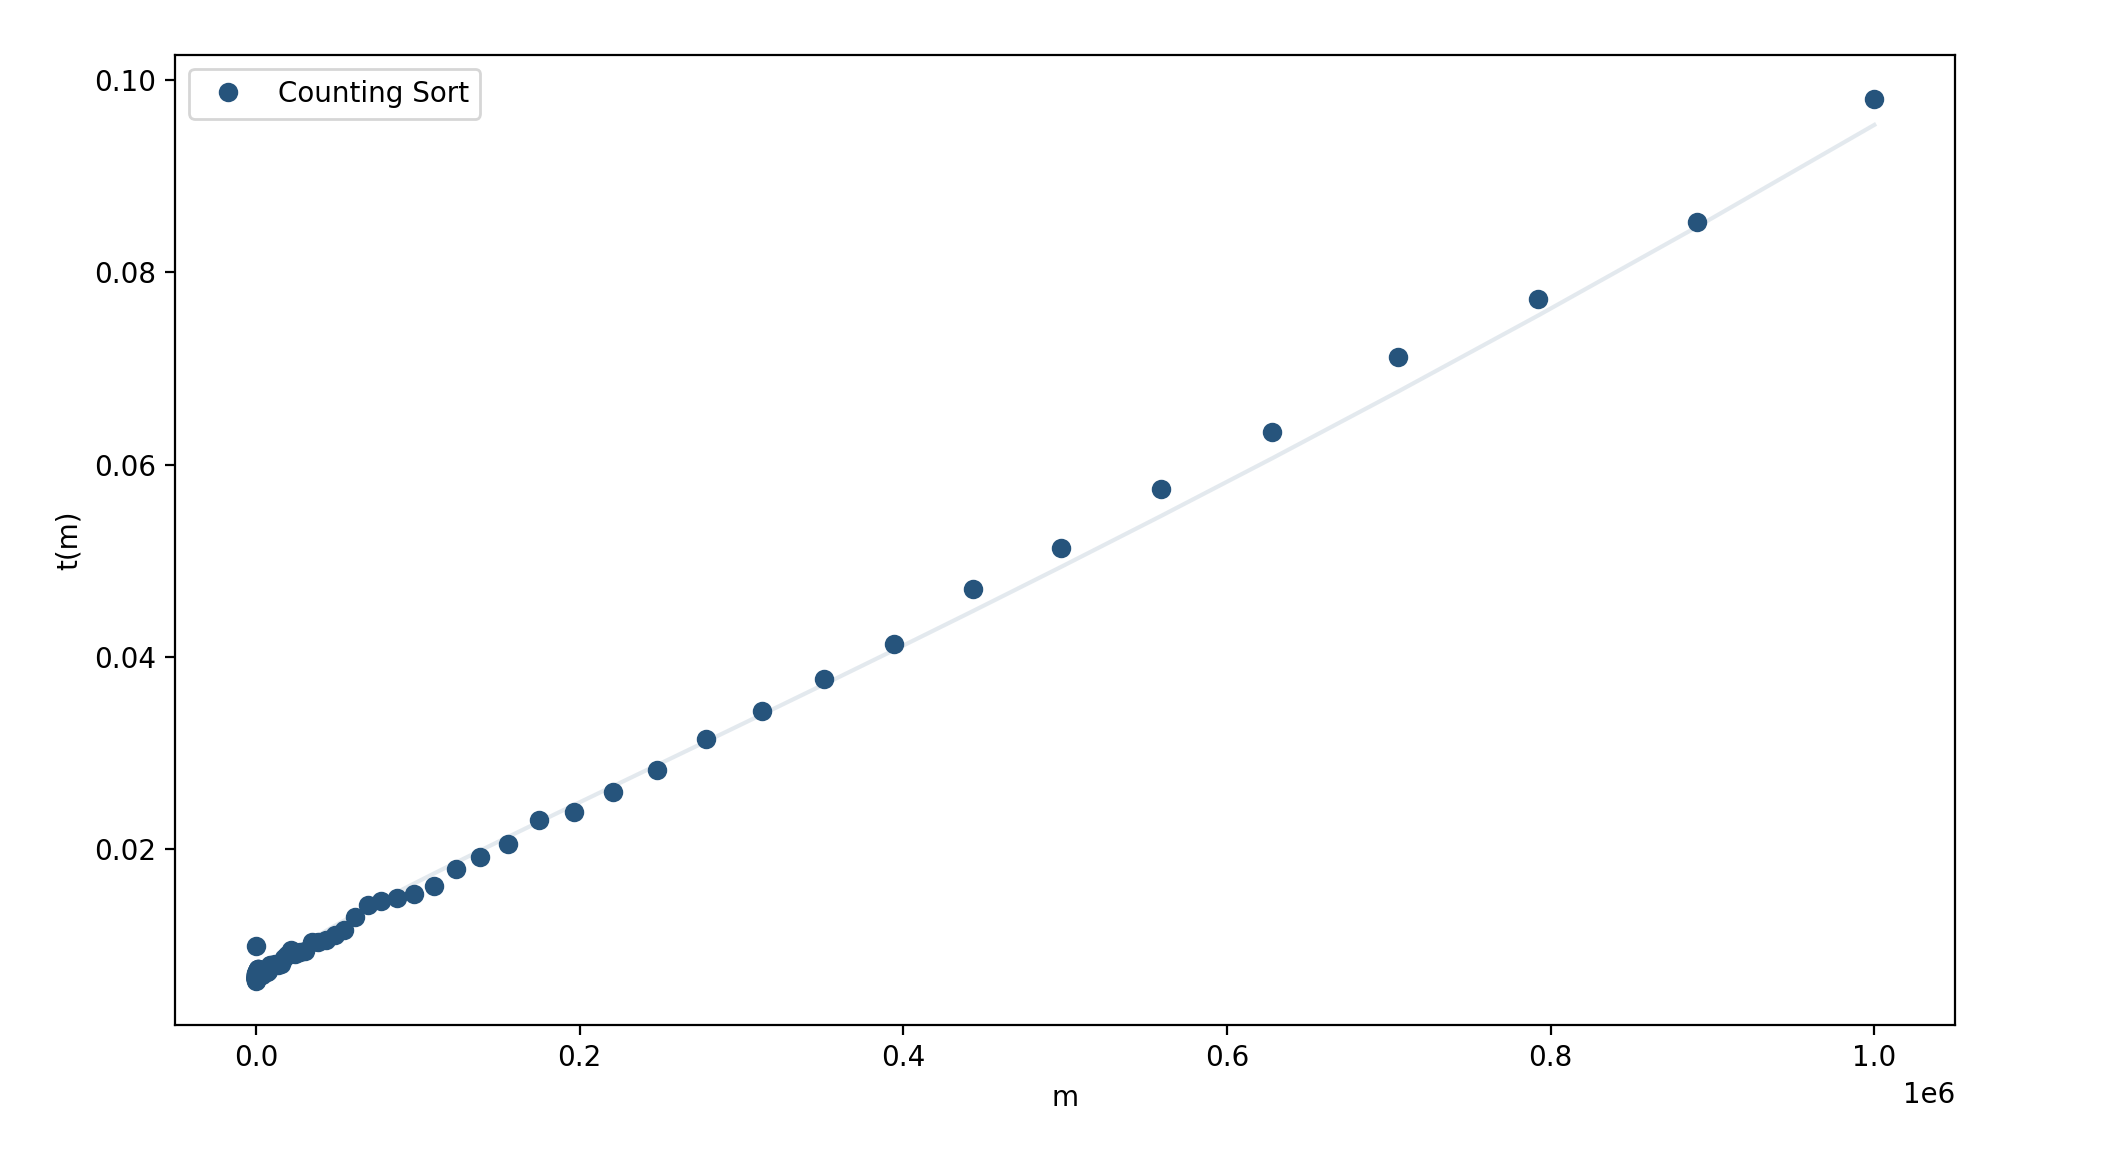
\includegraphics[width=0.9\textwidth]{images/grafico_counting_sort_m.png}
\end{center}



\chapter*{Quick Sort}
\addcontentsline{toc}{chapter}{Quick Sort}

Quick Sort è un algoritmo di ordinamento basato sulla tecnica del "divide et impera". L'idea principale è quella di selezionare un elemento pivot e partizionare l'array in due sottosequenze: gli elementi minori del pivot e quelli maggiori. Passaggi principali che effettua l'algoritmo:

\begin{enumerate}
	\item Si sceglie un elemento \textbf{pivot} dall'array.
	\item Si riordinano gli elementi in modo tale che tutti quelli minori del \textbf{pivot} lo precedano e quelli maggiori lo seguano.
	\item Si applica \textbf{ricorsivamente} Quick Sort alle due sottosequenze.
\end{enumerate}

\noindent Quick Sort è molto efficiente nella pratica, anche se nel caso peggiore ha una complessità quadratica.

\subsection*{Analisi della complessità}

La complessità temporale di Quick Sort è:
\begin{itemize}
	\item Caso medio: \(O(n \log n)\) 
	\item Caso peggiore: \(O(n^2)\)
	\item Caso migliore: \(O(n \log n)\)
\end{itemize}

\noindent Nella pratica, il caso peggiore si verifica raramente se si utilizza un buon criterio di scelta del pivot (es. pivot casuale o mediana di tre).

\subsection*{Grafico dei tempi di esecuzione}

Abbiamo generato un grafico in cui varia la lunghezza dell'array \textbf{n} da ordinare, mentre il paramentro \textbf{m} resta fisso. L'ordinamento viene eseguito con Quick Sort su array contenenti numeri casuali. Come ascissa abbiamo \textbf{n} da 100 a 1000000, e come ordinata il tempo di esecuzione in secondi.

\begin{center}
	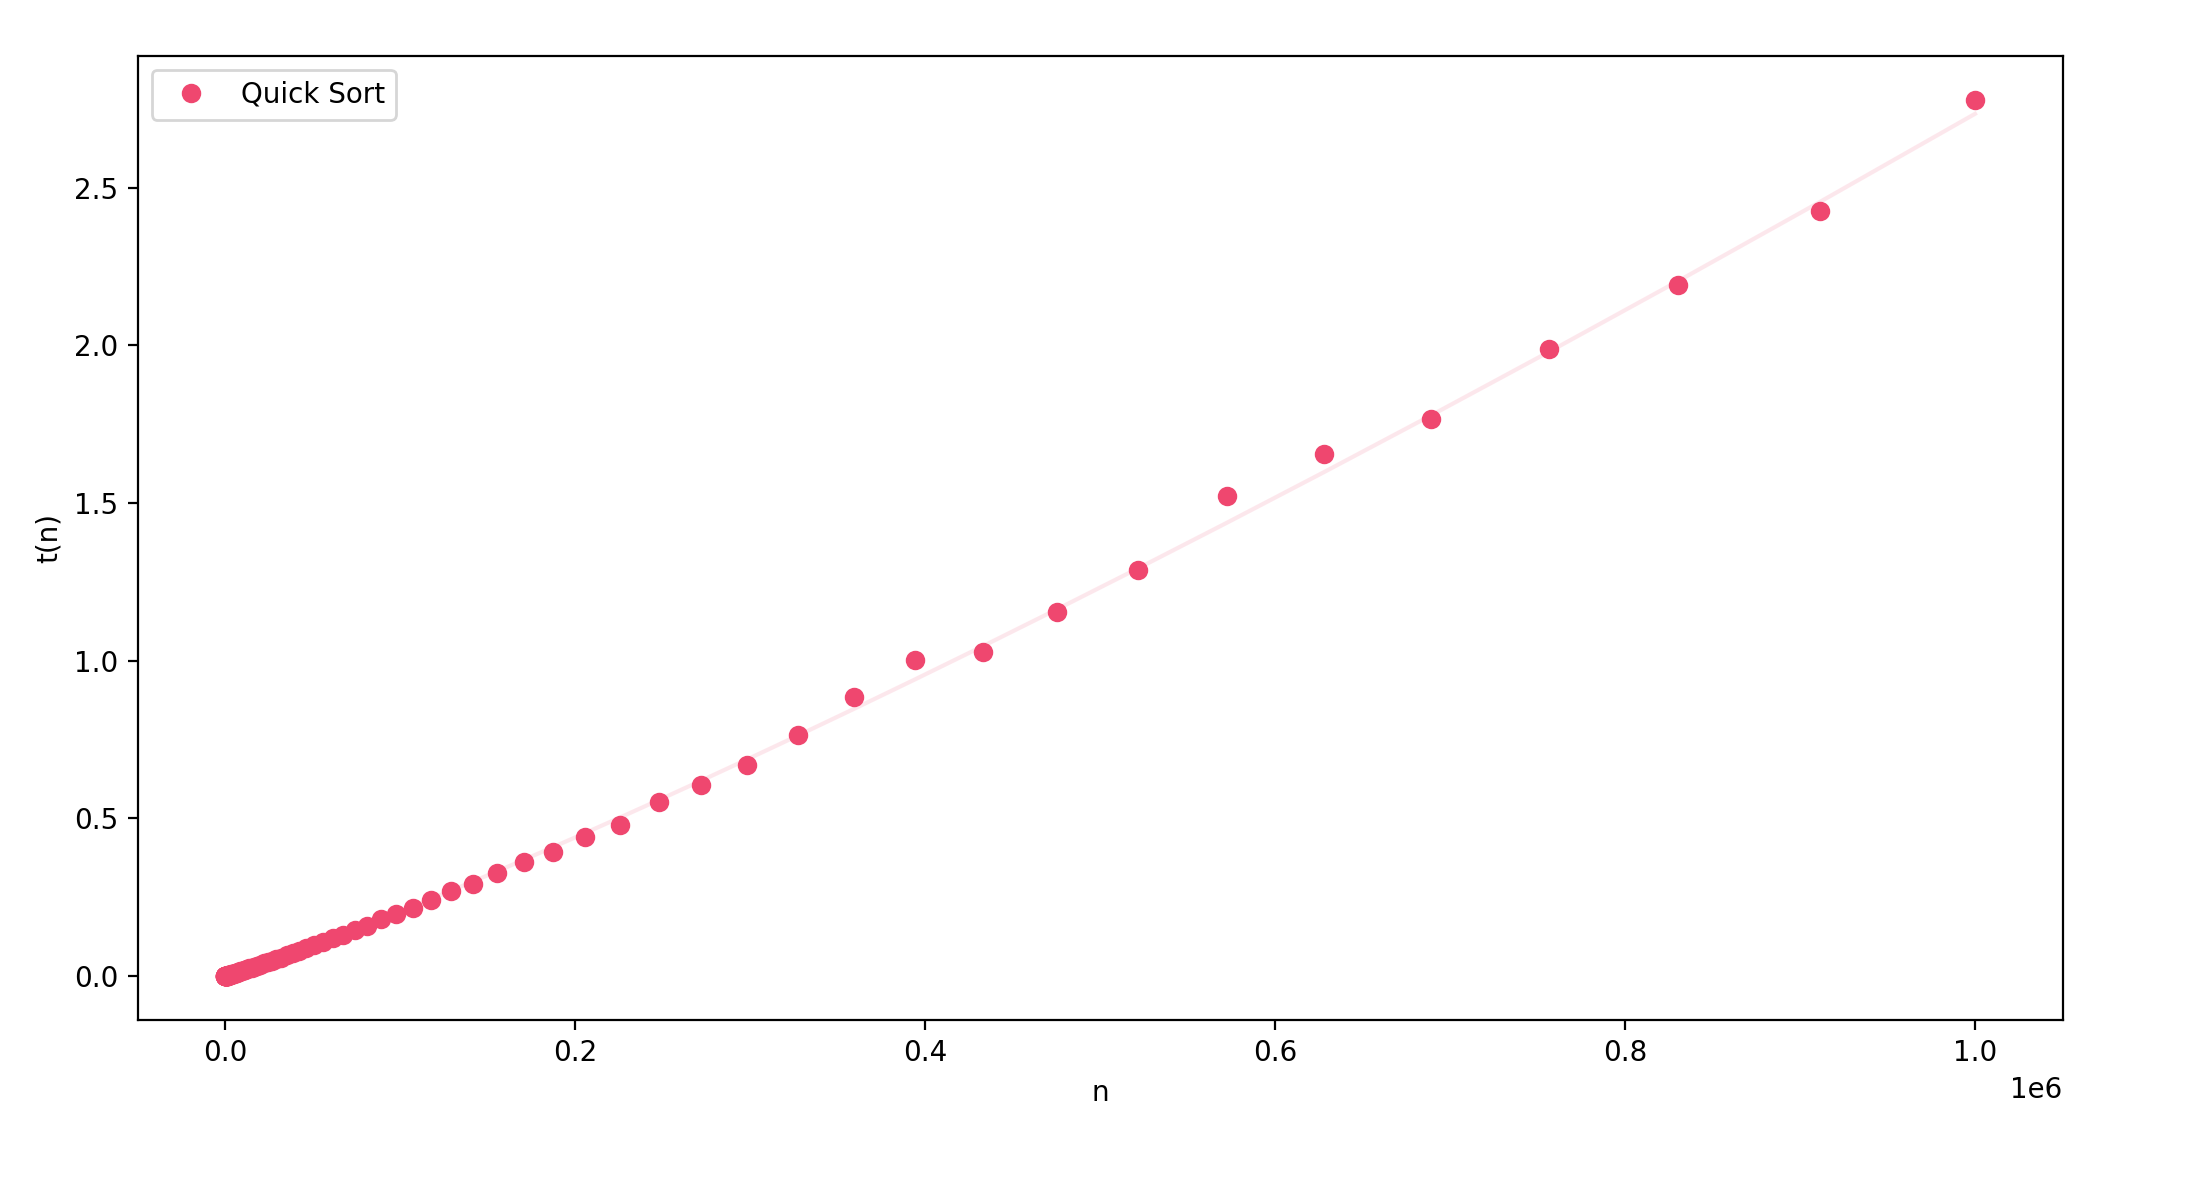
\includegraphics[width=0.9\textwidth]{images/grafico_quick_sort_n.png}
\end{center}

\noindent Successivamente, abbiamo realizzato un grafico in cui varia l'intervallo dei valori possibili presenti nell'array, (\textbf{m}), mantenendo costante la sua lunghezza a 10000 (\(n=10000\)). Nel grafico riportato qui sotto, sull'asse delle ascisse è rappresentata la variazione di \textbf{m} da 10 a 1000000 in scala scientifica (ogni valore va moltiplicato per \(10^6\)), mentre sull'asse delle ordinate è riportato il tempo di ordinamento dell'array in secondi.
 
\begin{center}
	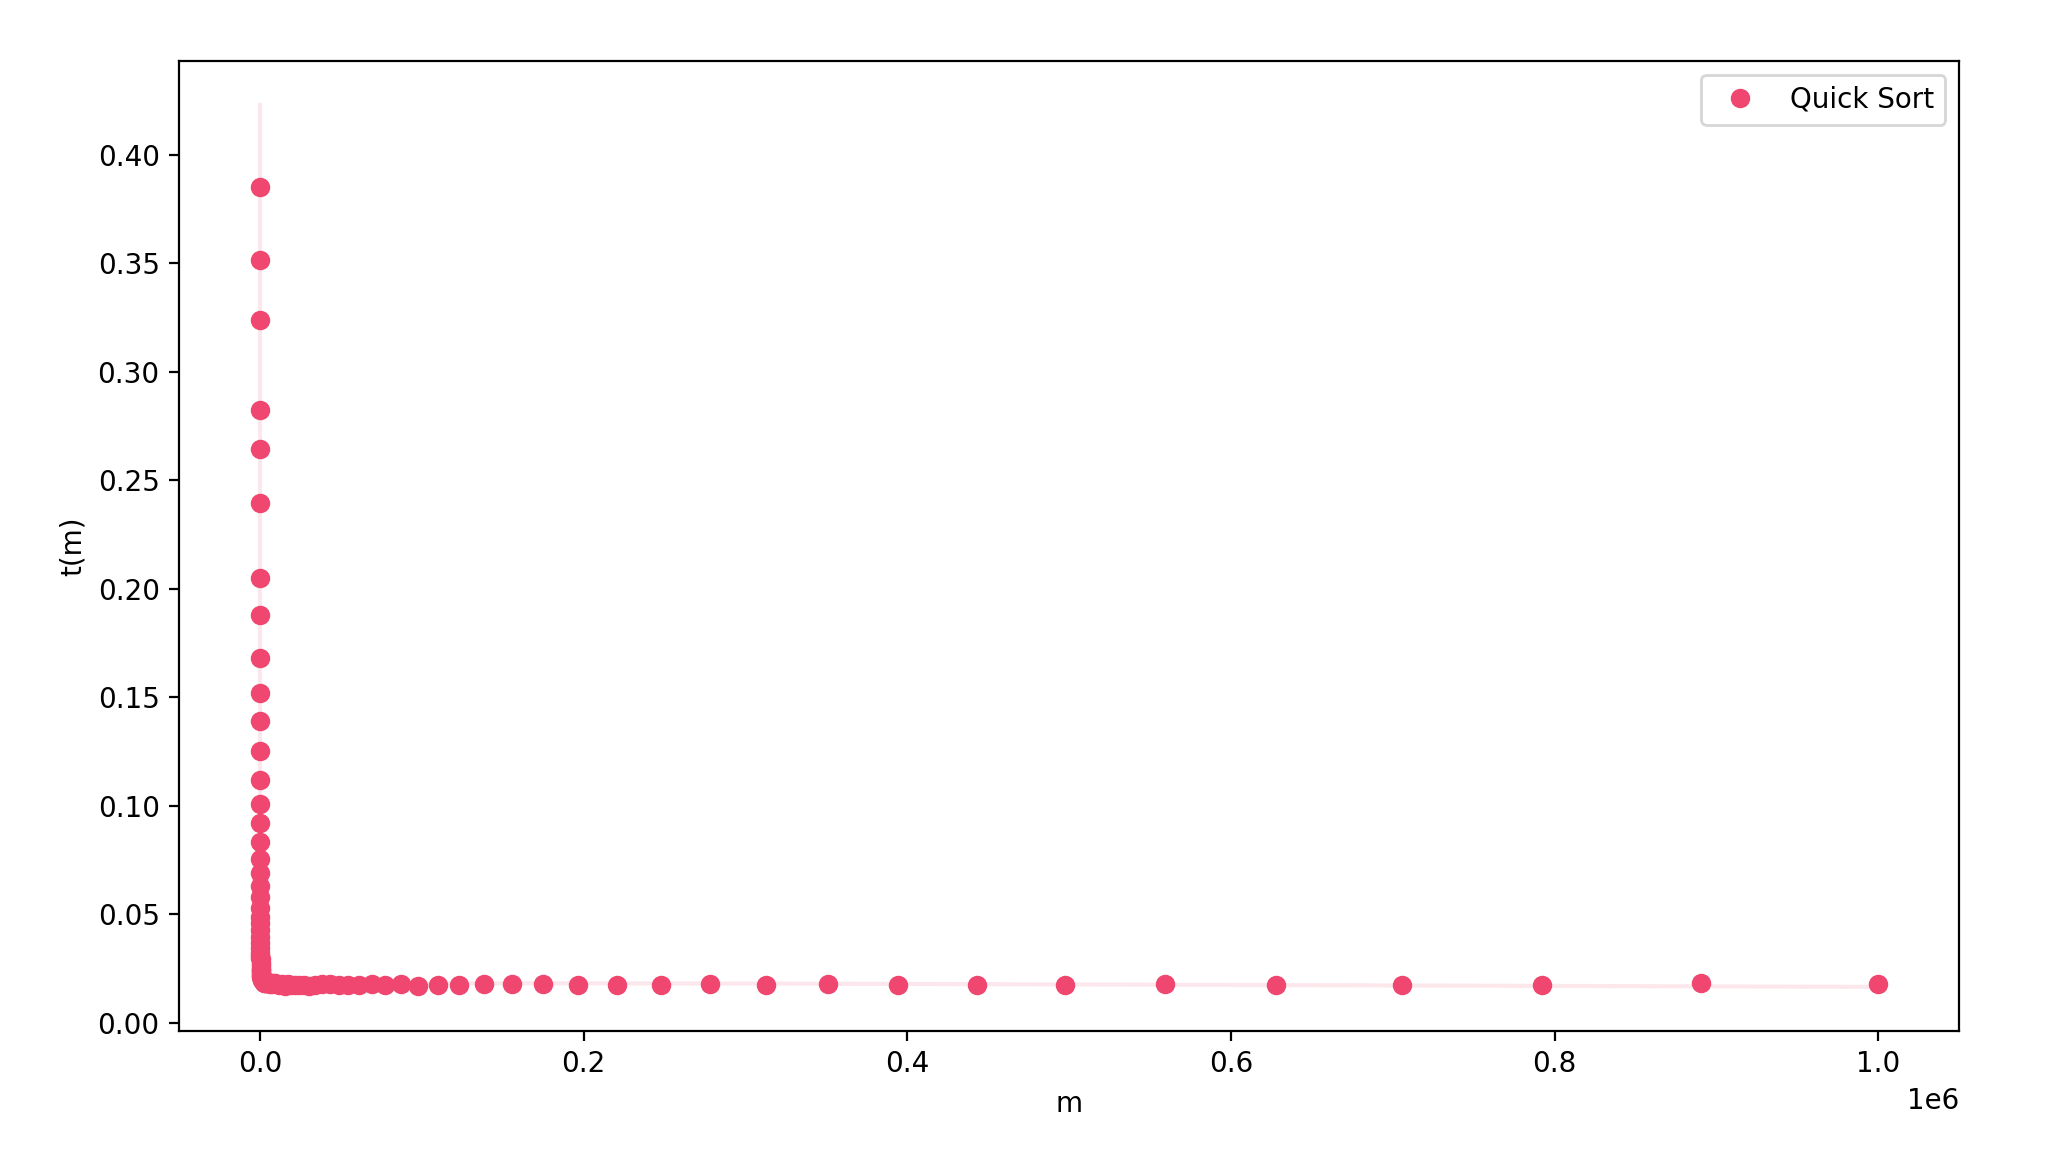
\includegraphics[width=0.9\textwidth]{images/grafico_quick_sort_m.png}
\end{center}

\noindent Qui si riscontra una problema nel grafico quando il numero di elementi possibile dell'array è molto basso, bisognerà indagare il motivo.

\chapter*{Quick Sort 3 Way}
\addcontentsline{toc}{chapter}{Quick Sort 3 Way}



\chapter*{Radix Sort}
\addcontentsline{toc}{chapter}{Radix Sort}

\chapter*{Conclusioni}
\addcontentsline{toc}{chapter}{Colusioni}


\end{document}
